\section{Implementering}

\subsection{Hardware}

Hardwaren på produktet er bygget fra bunden. Rammen som prototypen står på er taget fra et gammel metal-stel, men udover dette er resten konstrueret af gruppens medlemmer. Skinnerne er skåret i kabelføringsbakker og det samme er vognene. Alt er skruet og samlet af gruppen selv. 

Systemets PSoC'er er samlet under ét fordelingsprint. Dette print samler dataene fra PSoC-XY, -Z, og -Sensor og sender dem videre ud til enten motorerne eller sensorerne. 

% Fordelingsprint
\subsubsection{Fordelingsprint}
\begin{figure}[H] \centering
    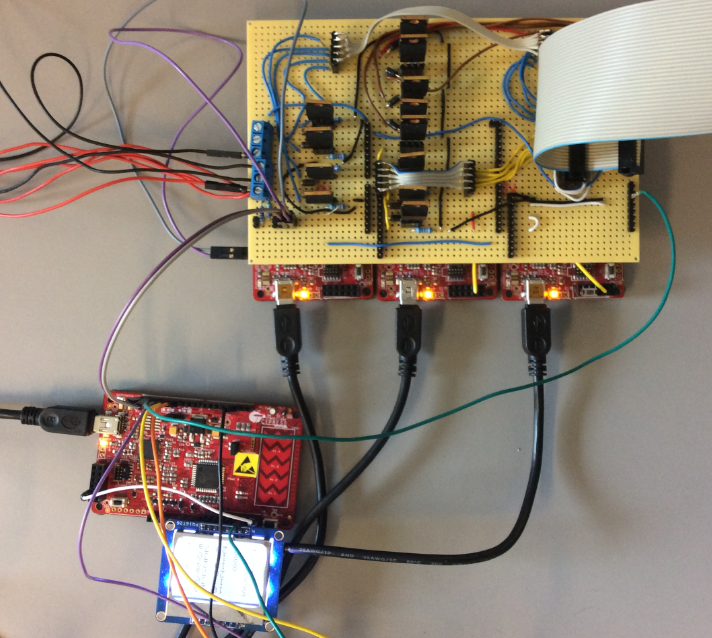
\includegraphics[width=0.6\textwidth]{Filer/FordelingsPrint.PNG}
    \caption{Fordelingsprint}
    \label{fig:Fordelingsprint}
\end{figure}

På figur \ref{fig:Fordelingsprint} ses fordelingsprintet. Dette print er bygget med pins så det kan sættes på XY-, Z- og Sensor PSoCs og dermed slippe for alt for mange ledninger. Printet indeholder hardwaren til I2C-kommunikation mellem PSoC-Master og de resterende PSoCs samt tre motorstyringer til henholdsvis X, Y og Z-motorerne. Derud over er printet forbundet med motorene, sensorerne og LED'erne\footcite{L-154A4} via. et 34 leder kabel.
For printlayout og diagram, Se dokumentationsrapporten\footcite{documentation}.

% X Moter Montering
\subsubsection{X Motor Montering}
\begin{figure}[H] \centering
    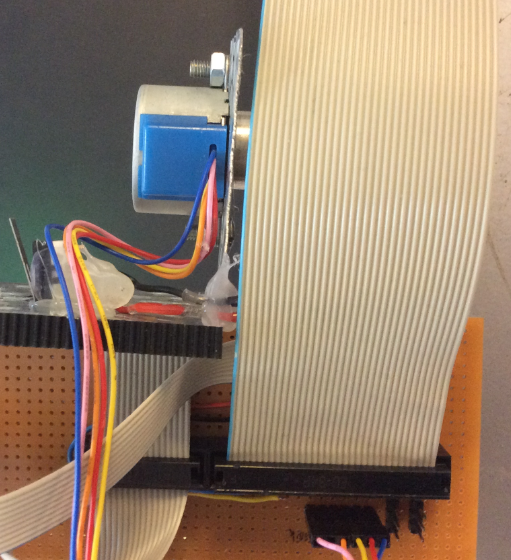
\includegraphics[width=0.5\textwidth]{Filer/XMotorMont.PNG}
    \caption{X Motor Montering}
    \label{fig:XMotorMont}
\end{figure}

På figur \ref{fig:XMotorMont} ses tilslutningen af 34 leder kablet fra fordelerprintet samt monteringen af den ene af X-motorerne. Fra denne tilslutning bliver signaler, spændinger og kommunikation fordelt ud til deres respektive enheder. For printlayout og diagram, Se dokumentationsrapporten\footcite{documentation}.

% Z Motor Montering
\subsubsection{Z Motor Montering}
\begin{figure}[H] \centering
    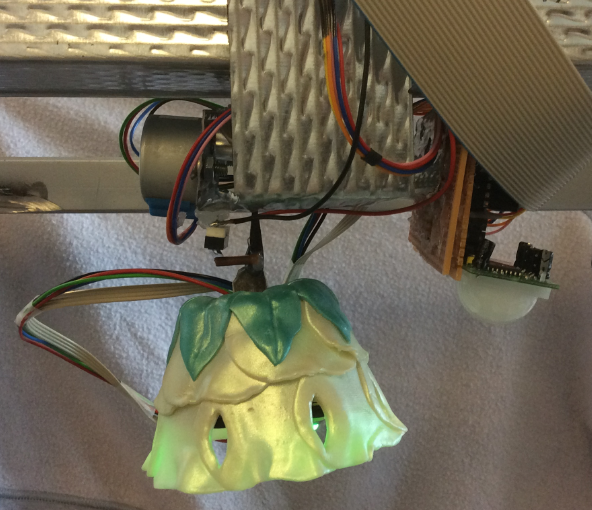
\includegraphics[width=0.6\textwidth]{Filer/ZMotorMont.PNG}
    \caption{Z Motor Montering}
    \label{fig:ZMotorMont}
\end{figure}

På figur \ref{fig:ZMotorMont} ses bunden af Z-vognen. Det er her Z-motoren, lampen med RGB dioder\footcite{L-154A4} samt systemets sensorer er monteret. For printlayout og diagram, Se dokumentationsrapporten\footcite{documentation}.

\subsection{Software}

I projektet er der brugt både C og C++. Alt PSoC software er skrevet i C da det er det sprog PSoC Creator understøtter. Desuden er SPI driveren til DevKit8000 skrevet i C, fordi den er skrevet som et Linux-kernemodul og det kræver igen C. Sidst men ikke mindst er GUI'en på DevKit8000 skrevet i C++ med brug af QT biblioteket.

\subsubsection{Devkit8000}

På Devkit8000 er de mest interessante moduler:

\begin{itemize}
	\item position
	\item light
	\item settings
\end{itemize}

\textbf{Position} er den kodesektion der beskriver hvordan lampen skal bevæge sig på de tre akser. Kodesektionen håndterer videreførelsen af de beskeder som brugeren opretter gennem position-fane. Det særligt interessante består i den grafiske repræsentation, bestående af et koordinatsystem, skal stemme overens med den reelle positionering af produktet. Således kan brugeren virtuelt blive repræsenteret for, hvordan systemet vil blive påvirket såfremt brugeren vælger at realisere disse ved at videresende vha. SPI.

\textbf{Light} er den kodesektion der beskriver lysstyringen for lampens RGB-LED'er\footcite{L-154A4}. På samme måde som ved position, viderekommunikeres brugeraktionen på de grafiske elementer til systemet, såfremt dette vælges af brugeren, og genererer desuden en virtuel repræsentation. I dette tilfælde repræsenteres værdierne med en farve palette med den blandede farve bestående af de tre værdier. Særligt interessant er det her, at præsentere for brugeren hvordan interaktionen påvirker systemet forinden det bliver viderebragt og påvirker lampens lys.

\textbf{Settings} kodesektionen står for den generelle sensorkontrol. Man kan her både ved bevægelsessensoren og lumensensoren betragte Devkit8000 som en afbryder, da disse kun kan ændres til to tilstande; tændt og slukket. Den sidste sensor der påvirkes i denne sektion er afstandssensoren, der altid er aktiv. Denne kan påvirkes med hensyn til hvilken afstand den skal alarmere resten af systemet. Brugeren får gennem denne sektion frirum til at til- eller fravælge sensorfunktionalitet og indstille på dem.

\subsubsection{Master}

Særligt interresant i softwaren på PSoC-Master er \verb+isr_spi_rx()+ og \verb+i2c_tx()+ funktionerne, da de er bærende element i hele funktionaliteten.

\subsubsection{SPI}

%TC:ignore
\lstinputlisting[language=C,caption={isr\_spi\_rx()},label={listing:isrspirx}]{Filer/isr_spi_rx.c}
%TC:endignore

\verb+isr_spi_rx()+ Listing \ref{listing:isrspirx} er en \verb+Interrupt service routine+ som afvikles ved modtagelse af data via SPI-busset. Det modtagede data bliver læst ind på en buffer fra SPI komponenten, hvorefter det deles op i en kommando og en værdi. Alt efter hvilken kommando der er modtaget fortages en defineret handling. 


\subsubsection{I2C}

%TC:ignore
\lstinputlisting[language=C,caption={i2c\_tx()},label={listning:i2ctx}]{Filer/i2c_tx.c}
%TC:endignore

\verb+i2c_tx()+ Listing \ref{listning:i2ctx} funktionen bruges til afsendelse af datapakker på I2C-bussen. Når funktionen kaldes sendes der en addresse, kommando og værdi. Kommandoen og værdien sættes ind i en buffer til afsendelse. I bufferen er der også tilføjet en \verb+Start of packet (SOP)+ byte og en \verb+End of packet (EOP)+ byte, disse sættes ind hhv først og sidst i bufferen og bruges af modtageren til at kontrollere om den fulde pakke er modtaget.
Herefter kaldes en \verb+I2CM_I2CMasterWriteBuf()+ med modtager adressen, bufferen til afsendelse, buffer størelsen og mode for afsenelse, som er komplet afsendelse her. Derefter afventer funktionen at pakken er blevet korrekt afsendt og derefter nustiller I2C komponemtets status.


\subsubsection{XY I2C}

%TC:ignore
\lstinputlisting[language=C,caption={I2CS\_I2C\_ISR\_ExitCallback()},label={listning:i2csi2cisrexitcallback}]{Filer/I2CS_I2C_ISR_ExitCallback.c}
%TC:endignore

\verb+I2CS_I2C_ISR_ExitCallback()+ Listing \ref{listning:i2csi2cisrexitcallback} er en \verb+Interrupt service rotine+ som automatisk kaldes efter der er modtaget en datapakke over I2C-bussen.
Det modtagede data lagres ind i en struct og alt efter hvilken kommando der er modtaget fortages en defineret handling. Efterfølgende nulstilles SPI komponentens status.

\subsubsection{X-, Y- og Z-Styringskode}

Styringen af systemets motorer foregår via PSoC-XY og PSoC-Z. Disse PSoC'ere har deres eget program, som styrer hvilken handling de skal tage. De modtager gennem I2C to variable; en kommando og en værdi. Disse variable bruger de til at identificere deres handlinger og igangsætte de definerede funktioner.  


Funktionerne er som følger: \newline
\verb+SetXPos(uint XVal);+  \newline
\verb+SetYPos(uint Yval)+   \newline
\verb+SetZPos(uint Zval)+   \newline
\verb+StepXForwards();+     \newline
\verb+StepXBackwards();+    \newline
\verb+StepYForwards();+     \newline
\verb+StepYBackwards();+    \newline
\verb+StepZForwards();+     \newline
\verb+StepZBackwards();+    \newline
\verb+CalibrateX();+        \newline
\verb+CalibrateY();+        \newline
\verb+CalibrateZ();+        \newline
\verb+CY_ISR(isr_X);+	    \newline
\verb+CY_ISR(isr_Y);+	    \newline
\verb+CY_ISR(isr_Z);+	    \newline



\textbf{StepForwards / StepBackwards}\newline 
Når en position bliver valgt på Devkit8000 er det PSoC-XY og PSoC-Z der skal sørge for at positionere lampen til den valgt placering. Kommando-variablen bruger den til at definere hvilken motor der skal aktiveres, og værdi-variablen bruger den til at finde ud af hvor den skal kører motoren hen. 

Hvis motoren befinder sig i position 100 på X-aksen, gemt i variablen xPos, og kommandoen for aktivering af X-motor, SetXPos(), bliver kaldt, samt værdien der bliver modtaget er 150, vil PSoC-XY trække sin nuværende position fra den modtagede værdi. 150 minus 100 giver 50. da 50 er et positivt tal, vil StepXForwards() blive kaldt med værdien 50, altså; StepXForwards(50);
Hvis den sendte værdi var 50, ville resultatet give -50. Her vil StepXBackwards() blive kaldt med værdien 50, altså; StepXBackwards(50);
Dette er gældende for motorstyringen på alle tre akser. 

\textbf{Calibrate();}\newline 
Dette funktionskald aktiverer X-motorerne i den ene retning. Når retningens grænse er nået, vil en fysisk afbryder blive aktiveret og herved levere besked gennem CY\textunderscore{}ISR(isr\textunderscore{}) til PSoC-XY om at den nedre grænse er nået. Herefter vil X-motorerne køre i den anden retning til de rammer den øvre grænse hvor endnu en afbryder bliver aktiveret. \newline 
De steps motoren tager imellem den nedre og øvre grænse bliver gemt i en værdi kaldet xMax. Motorens nuværende position ved den øvre grænse gemmes i en variabel kaldet xPos som bliver sat til 0. 
\newline 
Når xMax og xPos er sat, aktiveres Y-motorerne i den ene retning. Når retningens grænse er nået, vil en fysisk afbryder blive aktiveret og herved leverer besked til PSoC-XY om at den nedre grænse er nået. Herefter vil Y-motorerne køre i den anden retning til de rammer den øvre grænse hvor endnu en afbryder bliver aktiveret. 
\newline 
Her bliver antal steps Y-motorerne har kørt gemt i en variabel kaldet yMax, og motorens nuværende position bliver gemt i en variabel kaldet yPos som sættes til 0. 
\newline
Fremgangsmåden som PSoC-Z bruger til at kalibrere sine værdier med, er meget lig den PSoC-XY benytter. Den kører lampen ned med SetZForwards() til den får et interrupt af afstandssensoren. Ved dette interrupt er den nedre grænse nået, og PSoC-Z vender nu motorens retning, og tæller antal steps op til næste interrupt. Den gemmer antal steps mellem de to interrupts i zMax, stopper ved øverste interrupt og sætter sin position i zPos til 0.
Hermed er skinnernes længde målt ud, rummets dybte målt ud, lampens position er sat og systemet er nu kalibreret.

\textbf{CY\textunderscore{}ISR(isr\textunderscore{})}\newline 
Ved skinnernes ydre grænser og ved lampens topposition sidder der Micro switches monteret. Ved aktivering slutter disse en kreds der levere 5V på den definerede pin på PSoC'en. når denne sættes igang, aktiveres Interrupt Service Rutinen. Denne stopper motoren på den pågældende akse, og igangsætter motoren den modsatte vej med 50 steps. At motorerne kører 50 steps tilbage er vigtigt for ikke at hvile på kontakten og have en konstant aktiveret interrupt der forhindre programmet i at gøre andet. 



% Sensor
\subsubsection{Sensor}

I PSoC-Sensor er de mest interessante moduler:

\begin{itemize}
	\item handler
	\item LumenSensor
	\item main
\end{itemize}

Modulet \textbf{handler} håndterer PSoC-Sensors opførsel når den modtager I2C kommandoer fra PSoC-Master. Basalt set én stor switch, med en case for hver kommando PSoC-Sensor kan modtage og håndtere.

\textbf{LumenSensor} er det software modul der håndterer I2C kommunikationen med lyssensoren. Dette har fået sit eget modul da en enkelt aflæsning af sensoren består af at skrive en byte til sensoren, læse to bytes fra sensoren, og derefter skrive en og læse to bytes igen.

 \textbf{main} indeholder den overordnede kontrolstruktur i PSoC-Sensor, der bestemmer hvornår alt andet skal køres. Som beskrevet ovenfor i TopDesign, så er hjertet Metronom timeren der giver et taktslag hver halve sekund. For hvert taktslag bliver en række tællere talt op og tjekket for overløb. Hver tæller der løber over bliver nulstillet og hæver et flag. De flag bliver tjekket i hoved-løkken og den tilhørende kode bliver udført.

Alt i alt gør denne opbygning at der kan defineres periodiske events med individuelle perioder (med en opløsning på 0.5 sekunder). Det giver den fordel at vi kan have en hoved-løkke der kører hele tiden, uden at blive standset af delay kommandoer, hvilket giver muligheden for et mere responsiv og jævnt kørende program. Men samtidig undgår vi at overbelaste sensorene ved at aktiverer dem alt for ofte.

Til sidst bør det nævnes at systemet bruger et \textbf{lux} modul som vi ikke har skrevet selv. Den er kopieret fra lumen sensorens datablad\footcite{TSL2561}.
